\chapter{Implementation of Bayesian Network Correction } \label{app:bnc}

We implemented the URSA algorithm described by \cite{Lee2013}.  Before we proceed, we introduce the notation used in this Appendix for describing our implementation:
\begin{itemize}
\item $i := $ the index of a label
\item $Y_i := $ a latent random variable corresponding to whether to assign label $i$ to the sample
\item $\tilde{Y}_i := $ random variable corresponding to the distribution over classifier scores for label $i$ 
\item $\bold{P}_i := $ set of parent of $Y_i$
\item  $\bold{C}_i := $ set of children random variables of $Y_i$ that are also latent random variables. That is, all children of $Y_i$ except for $\tilde{Y}_i$
\item  $\bold{S}_i := $ set of all parents of all random variables in the set $\bold{C}_i$ except for $Y_i$
\item $\bold{A}_i := $ set of all ancestors of $Y_i$
\end{itemize}
We note that bold random variables highlight the fact that the random variable is a set of random variables. We let the lowercase version of these random variables denote the value for a realization of the corresponding random variable (e.g. $X = x$). We also let $p(x)$ be shorthand for $p(X = x)$, the probability (if $X$ is discrete) or density (if $X$ is continuous) that random variable $X$ equals $x$. 


\section{Estimation of classifier output distributions }

For a given cell type $i$, we estimate the conditional distribution of the classifier's output $\hat{y}_i$ (distance to the decision boundary) conditional on its true label $y_i$ as a discrete random variable constructed by binning the classifier outputs  $\hat{y}_i$ as output in a 2-fold cross-validation process. Specifically, we partition the training data for cell type $i$ into two folds ensuring that no study is split between folds while attempting to keep the sizes of the two folds as similar as possible. We then train on one fold and compute the classifier scores from the second fold (for each of the two folds).

Using all of these scores, we then estimate a histogram using a second 2-fold cross-validation scheme. We compute the width of the histogram using the range of scores. We then test a number of bin sizes by first estimating a histogram density function using data in one fold and then computing the likelihood of the data in the second fold (performing this procedure for both folds). The histogram density function is given by
$$f(x) := \frac{1}{nh}\text{Count}(x) $$
where $n$ is the total number of data points, $h$ is the width of each bin, and $\text{Count}(x)$ is the number of data points sharing the same bin as $x$. 
We choose a bin size that maximizes the mean of the two data log likelihoods computed on each fold.


\section{Estimation of the prior distribution }

As described by Lee \textit{et al.} (2013), the true cell type assignments $p(y_1, \dots, y_n)$ factor according to the ontology graph:
$$p(y_1, \dots, y_n) := \prod_{i=1}^m p(y_i \mid \bold{c}_i)$$
These conditional distributions $p(y_i \mid \bold{c}_i)$ enforce consistency with the ontology:
 $$p(Y_i=1 \mid \bold{c}_i) := \left\{
     \begin{array}{lr}
       1.0 & : 1 \in \bold{c}_i   \\
       \text{prior}_i & : \text{otherwise}
     \end{array}
     \right.$$
The $\text{prior}_i$ values are computed from counts in the training data. Specifically, the prior for each leaf-node cell type $\ell$ is simply the fraction of samples in the data set labelled as $\ell$.  For each internal node $\ell$, the prior is computed as the fraction of all samples  labelled as $\ell$, but not labelled as any child of $\ell$. A pseudocount of one was used in the calculation for all priors.

\section{Gibbs sampling algorithm }

Gibbs sampling is a member of a family of techniques, called Markov chain Monte Carlo (MCMC), for sampling from a complex joint probability distribution. Given a joint distribution over a set of random variables $P(\bold{X})$ where $\bold{X} := \{X_1, \dots, X_n\}$, Gibbs sampling involves first initializing all of the random variables to some preset values and then iteratively sampling each random variable from its distribution conditioned on the current values of the remaining random variables (Algorithm~\ref{algo:gibbs}). As the number of iterations approaches infinity, the samples from this procedure will approach the target joint distribution. Of course, in practice, only a finite number of samples can be obtained; however, with sufficient numbers of samples, an approximate estimate can be obtained. Usually, some number of initial samples are discarded in order for the Markov chain to approach its stationary distribution, at which point, the sampling distribution will more closely resemble the target distribution. In order to implement Gibbs sampling, one must be able to sample from each random variable conditioned on the remaining random variables.

\begin{algorithm}
\caption{Gibbs Sampling}
\label{algo:gibbs}
\begin{algorithmic}
\State $t \gets 0$
\For{$i = 1, \dots, n$}
	\State $x_i^{(t)} \gets \text{Some, possibly random, initial and valid value for } X_i$
\EndFor
\For{$t = 1, \dots, T$}
	\For {$i = 1, \dots, n$} 
		\State $x_i^{(t)} := x_i^{(t-1)}$
	\EndFor
	\For {$i = 1, \dots, n$}
		\State $x_i^{(t)} \sim p(x_i \mid \bold{x}^{(t)} \setminus x_i^{(t)})$
	\EndFor
\EndFor
\end{algorithmic}
\end{algorithm}

In Bayesian networks, each random variable's Markov blanket consists of its parents, its children, and it's children's parents. In the Bayesian network for BNC, each conditional distribution can therefore be computed using:
\begin{align*}
p(y_i \mid \tilde{y}_i, \bold{s}_i, \bold{c}_i, \bold{p}_i) &\propto p(y_i, \tilde{y_i}, \bold{s_i}, \bold{c}_i, \bold{p_i}) \\
&= p(\tilde{y}_i \mid y_i) p(y_i \mid \bold{p}_i) p(\bold{c}_i \mid y_i, \bold{s}_i)  \\
&= p(\tilde{y}_i \mid y_i) p(y_i \mid  \bold{p}_i)  \prod_{y_j \in \bold{c}_i} p(y_j \mid y_i, \bold{p}_j \setminus y_i)\\
&=  \left\{
     \begin{array}{lr}
       p(\tilde{y}_i \mid y_i) p(y_i \mid  \bold{p}_i)  \prod_{y_j \in \bold{c}_i} p(y_j \mid y_i, \bold{p}_j \setminus y_i)  : y_i = 1  \\
       p(\tilde{y}_i \mid y_i) p(y_i \mid  \bold{p}_i)  \ \ \ \ \ \ \ \ \ \ \ \ \ \ \ \ \ \ \ \ \ \ \ \ \ \ \ \ \ \  \ \ \ \ \ \ \ \ \ \ \ \ : y_i = 0
     \end{array}
   \right.
\end{align*}
where the normalizing constant is
$$Z := \left[\sum_{y_i \in \{0,1\}} p(\tilde{y}_i \mid y_i) p(y_i \mid  \bold{p}_i) \prod_{y_j \in \bold{c}_i} p(y_j \mid y_i, \bold{p}_j \setminus y_i) \right]^{-1}$$


The construction of the Bayesian network in BNC admits a fast Gibbs sampling algorithm.  This algorithm relies on the observation that if, during the course of Gibbs sampling, a given node has any parent that is assigned (i.e. equal to one), then this node will also be assigned with probability one. Therefore, there is no need to explicitly sample this node. Similarly, if a node has any child that is unassigned (i.e. equal to zero), then this node will also be unassigned with probability one.  This observation leads to a sped up Gibbs sampling algorithm that avoids sampling every random variable on each iteration (Algorithm~\ref{algo:gibbs_bnc}).  In this algorithm, the nodes are visited according to the topological order of the DAG and a set is maintained that keeps track of those nodes that do not need to be explicitly sampled on their next visit.  When a node changes its assignment value (from zero to one, or one to zero), the set of skippable nodes is updated (Fig.~\ref{fig:gibbs_bnc}).

\begin{figure*}[!tpb]
\centerline{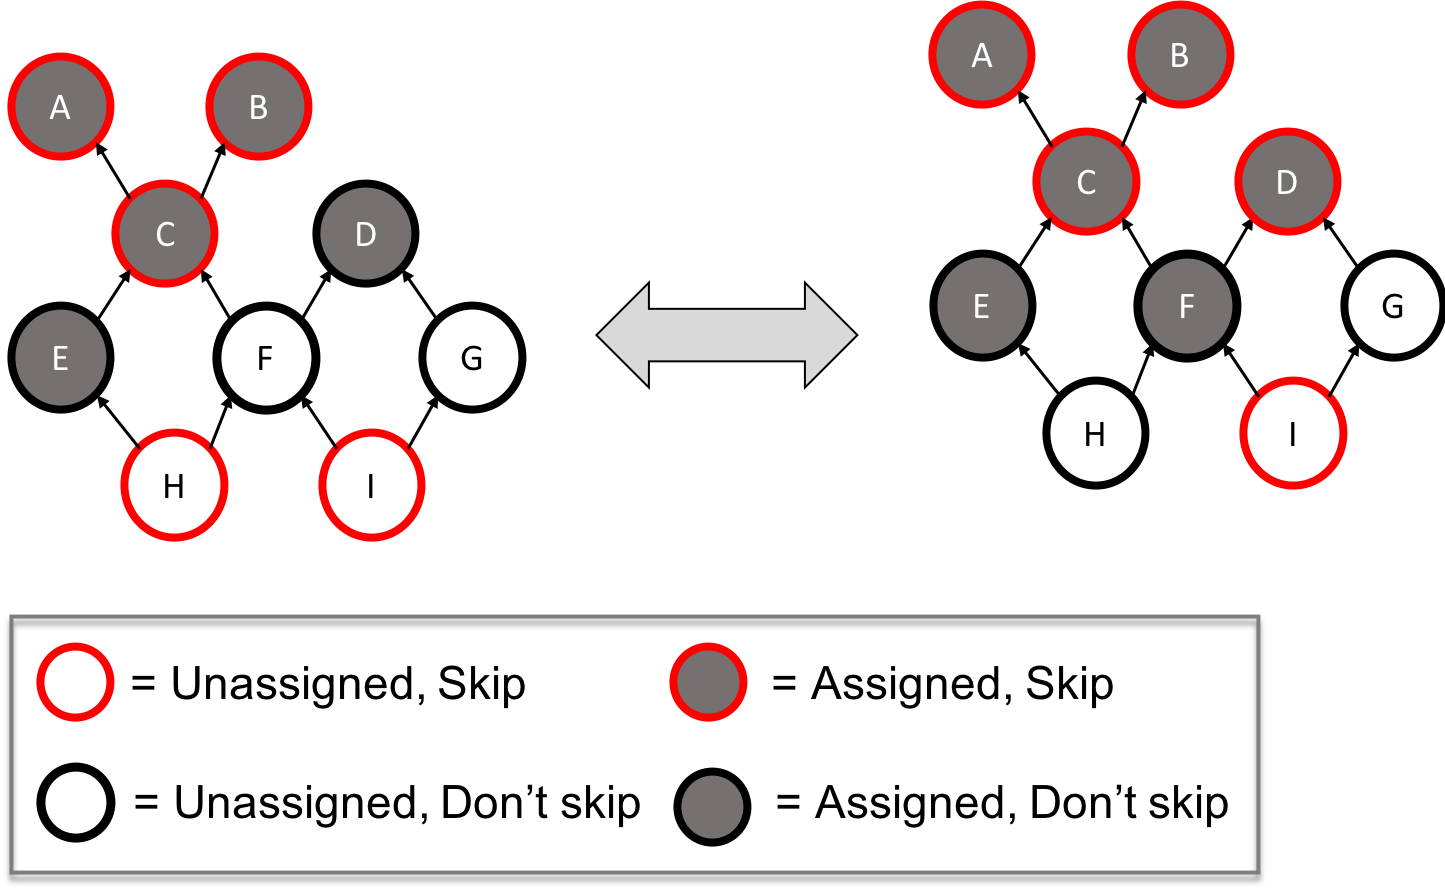
\includegraphics[width=11cm]{figures/gibbs_bnc.png}}
\caption{\textbf{Gibbs sampling for BNC.} An example depicting a step in the BNC Gibbs sampling algorithm. The node labelled "F" has either switched from unassigned to assigned (left-to-right) or from assigned to unassigned (right-to-left). Upon switching its assignment, the algorithm updates the set of nodes for which sampling does not need to be performed explicitly upon their next visit (nodes circled red).}
\label{fig:gibbs_bnc}
\end{figure*}

\begin{algorithm}
\caption{Gibbs Sampling for Bayesian Network Correction}
\label{algo:gibbs_bnc}
\begin{algorithmic}
\Procedure{GibbsForBNC}{$L, T$} \Comment{$L$ is the set of latent variable nodes in the DAG. $T$ is the number of iterations to run Gibbs sampling.}
\State $\text{Skip} \gets \emptyset$ \Comment{The set of random variables that don't require sampling}
\State $\bold{y}^{(0)} \gets \Call{Initialize}{L}$ \Comment{Initialize the random variables to some configuration that is consistent with the DAG.}
\State $\text{Pos} \gets \left\{y^{(0)} \in \bold{y}^{(0)}  \mid y^{(0)} = 1\text{}  \right\}$
\State $\boldsymbol{\ell} \gets \Call{TopologicalSort}{L}$ \Comment{Sort the nodes topologically according to the DAG.}
\For {$t = 1, \dots, T$}
	\For {$i \in L$} 
		\State $y_i^{(t)} \gets y_i^{(t-1)}$
	\EndFor
	\For {$i = \ell_1, \dots, \ell_{|L|}$}
		\If {$i \notin \text{Skip}$}
			\State $y_i^{(t)} \sim p\left(y_i \mid \tilde{y}_i, \bold{s}_i^{(t)}, \bold{c}_i^{(t)}, \bold{p}_i^{(t)}\right)$		
			\State $\Call{UpdateSkip}{y_i^{(t)}, y_i^{(t-1)}, \text{Skip}, \text{Pos}}$
		\EndIf
	\EndFor
\EndFor
\EndProcedure
\item[]
\Function{UpdateSkip}{$y_i^{(t)}, y_i^{(t-1)}, \text{Skip}, \text{Pos}$}
 	\If {$y_i^{(t)} = 1$ \textbf{and} $y_i^{(t-1)} = 0$} \Comment{The node went from unassigned to assigned}
		\State $\text{Pos} \gets \text{Pos} \cup \{i\}$
		\State $\text{Skip} \gets \text{Skip} \cup \text{children}(i)$ 		
		\For {$j \in \text{parents}(i)$}
			\If {$\text{children(j)} \subseteq \text{Pos}$}
				\State $\text{Skip} \gets \text{Skip} \setminus \{j\}$
			\EndIf	
		\EndFor
	\EndIf
	\If {$y_i^{(t)} = 0$ \textbf{and} $y_i^{(t-1)} = 1$}  \Comment{The node went from assigned to unassigned.}
		\State $\text{Pos} \gets \text{Pos} \setminus \{i\}$
		\State $\text{Skip} \gets \text{Skip} \cup \text{parents}(i)$
		\For {$j \in \text{children}(i)$} 
			\If {$\text{parents(j)} \subseteq L \setminus \text{Pos}$}
				\State $\text{Skip} \gets \text{Skip} \setminus \{j\}$
			\EndIf
		\EndFor
	\EndIf
\EndFunction
\end{algorithmic}
\end{algorithm}

